\RequirePackage{luatex85,shellesc}
\documentclass[crop,tikz]{standalone}
\usepackage{pgfplots}
\usepackage{ifthen}
\usepackage{circuitikz}

\usetikzlibrary{calc,arrows,arrows.meta}
\begin{document}

\newcommand\SWITCH[6]{ % name, x, y, width, rotation, on-off
    \edef\y{0.2}
    \ifthenelse{#6=1}{\edef\y{0.1}}{}
    \begin{scope}[xshift=-#2, yshift=-#3, rotate=#5]
        \draw[-Circle,line width=#4] (0 cm,0 cm) node (#1_a) {} -- (1 cm,0);
        \draw[Circle-,line width=#4] (1.5 cm,0) -- (2.5 cm,0) node (#1_b) {};
        \draw[line width=#4] (1 cm,\y cm) -- (1.5 cm,\y cm);
        \draw[line width=#4] (1.25 cm,\y cm) -- ++(0,0.2 cm);
    \end{scope}
}

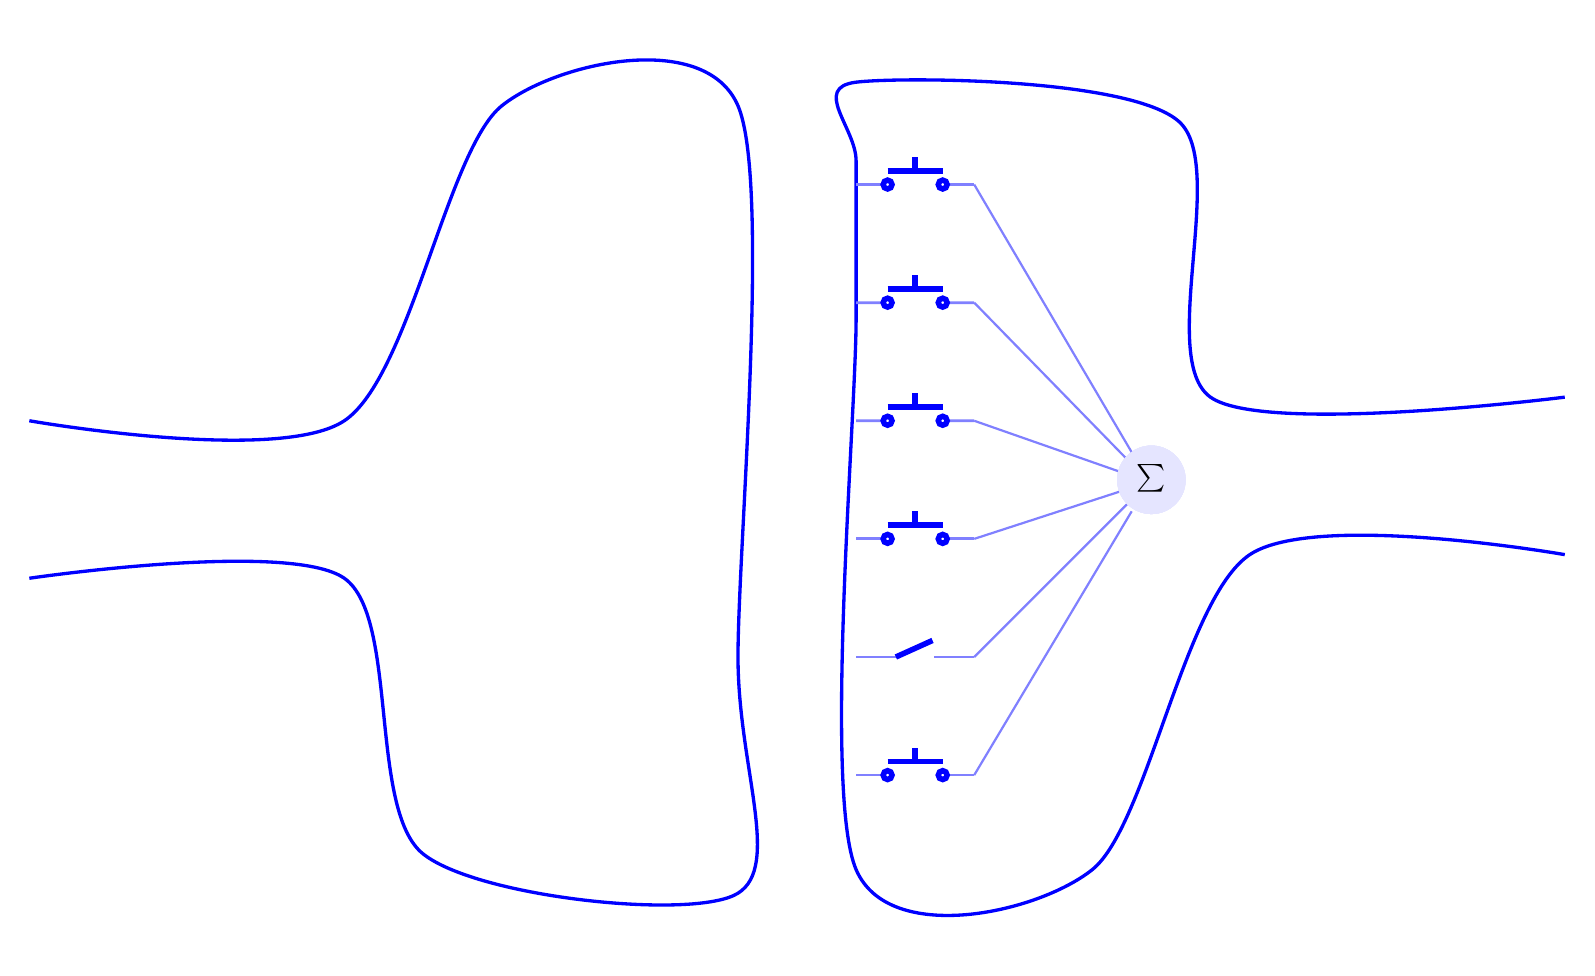
\begin{tikzpicture}[scale=1 , every node/.style={} ]
    
    % Draw synapse.
    \begin{scope}[rotate=-90]
        \draw[color=blue,very thick] plot[smooth] coordinates { 
            (-3, -8) (-3, -4) (-7, -2) (-7,1) 
            (0, 1) (3,1) (2.5,-3) (-1,-4) (-1,-8) 
        };
    \end{scope}

    \begin{scope}[yshift=4.3cm, xshift=3.5cm, rotate=90]
        \draw[color=blue,very thick] plot[smooth] coordinates { 
            (-3, -8) (-3, -4) (-7, -2) (-7,1) 
            (0, 1) (2,1) (3,1) (2.5,-3.1) (-1,-3.5) (-1,-8) 
        };
    \end{scope}

    % switches
    \foreach \y in {-1.5,0,1.5,3,4.5,6}
    {
        \edef\CLR{blue!50}
        \pgfmathsetmacro{\LW}{1}
        \pgfmathsetmacro{\AA}{rnd}
        \ifdim\AA pt<0.7pt
            \draw[line width=\LW pt, \CLR, smooth] (2.5,\y) to[push button,
                color=blue] (4,\y);
        \else
            \draw[line width=\LW pt, \CLR, smooth] (2.5,\y) to[nos,
                color=blue] (4,\y);
        \fi

        % path.
        \draw[color=\CLR, thick ] plot[smooth] coordinates {
            (4,\y) (6,2+0.1*\y) 
        };

        \node[fill=blue!10,circle] at (6.25,2.25) {\Huge $\sum$};

    }
    % integrator


\end{tikzpicture}	


\end{document}

